\chapter{Results}

\section{Statistical analysis}

\subsection{Systematic uncertainties}

This section covers the systematic, including statistical, errors associated with the analyis. The general strategy is to duplicate the systematics applied in the SM H to 4l search, including errors on the background estimation from data, and add the errors associated with MET modelling, guided by the mono-H to $\gamma\gamma$ strategy. 

% Uncertainties
\subsubsection{Uncertainties on Reducible Background estimation} %using Opposite-Sign leptons}
\label{sec:zxUncert}

Sources of systematic uncertainties for the methods presented above
potentially arises from the different composition of background processes 
($DY$, $t \bar{t}$, $WZ$, $Z\gamma$) in the region where we measure and 
where we apply the fake ratios.
OS method corrects for the resulting bias via the ``3P1F component"
of its prediction. SS method corrects explicitly the electron fake rates
for the correct fraction of photon conversions, but no attempt is made 
to correct the muon fake rates.
The closure tests presented here are used to assess a possible residual
bias in the methods.

\paragraph{Statistics in 4l Control Sample}
The limited size of the samples in the control regions where we measure and where we apply the fake ratios is the source of the statistical uncertainties of the method. The dominating statistical uncertainty is driven by the number of events in the control region and is typically in the range of 1-10\%.

\paragraph{Sensitivity of Fake Ratios to Background Composition}
Compositions of reducible background processes ($DY$, $t \bar{t}$, $WZ$, $Z\gamma^{(*)}$) in the region where we measure and where we apply the fake ratio method are typically not the same. This is the main source of the systematic uncertainty of the fake ratio method.

This uncertainty can be estimated by measuring the fake ratios for individual background processes in the $Z+1L$ region in simulation. The weighted average of these individual fake ratios is the fake ratio that we measure in this sample (in simulation). The exact composition of the background processes in the 2P+2F region where we plan to apply the fake ratios can be determined from simulation, and one can reweigh the individual fake ratios according to the 2P+2F composition. The difference between the reweighed fake ratio and the average one can be used as a measure of the uncertainty on the measurement of the fake ratios. The fake ratios for individual processes, the average fake ratio and the reweighed fake ratio determined by simulation are shown in table below. The effect of this systematic uncertainty is propagated to the final estimates, and it amounts to about 32\% for $4e$, 33\% for $2e2\mu$ and 35\% for $4\mu$ final state. 

% \begin{table}[h]
% \scriptsize
%     \centering
%     \caption{
%     The fake ratios for individual background processes, the average fake ratio and the fake ratio reweighed according to the composition of backgrounds in 2P+2F region.}  
    
%     \begin{tabular}[!htb]{| l | c | c | c | c | c | c |} \hline
% Sample				& Light Jets		  & HF Jets& From $\gamma$ conv	    & average (in $Z+1\ell$) & reweighed (2P2F)	& uncertainty \\ \hline \hline
% electron fake ratio	& $0.012^{+0.001}_{-0.001}$ 	& $0.115^{+0.005}_{-0.006}$  & $0.293^{+0.043}_{-0.043}$  &$0.021^{+0.001}_{-0.001}$& $0.024^{+0.004}_{-0.004}$& 15\%    \\ 
% muon fake ratio 	& $0.057^{+0.003}_{-0.003}$ 	& $0.225^{+0.008}_{-0.008}$ & $0.003^{+0.455}_{-0.003}$ &$0.120^{+0.004}_{-0.004}$& $0.105^{+0.020}_{-0.017}$ & 13\% \\  \hline
% 	\end{tabular}
%     \label{tab:uncertFR}
% \end{table}

\paragraph{Shape Uncertainty}
In order to estimate the uncertainty on the $m_{4l}$ shape we have looked at the differences between the shapes of predicted background distributions for all three channels, and between both of the two methods. The envelope of differences between these shapes of distributions is used as an estimate of the shape uncertainty. The uncertainty is estimated to be roughly in the range of 5\% - 15\%. Since the difference of the shapes slowly varies with $m_{4l}$, it is taken as a constant versus $m_{4l}$  and is absorbed in the much larger uncertainty on the predicted yield of backgrounds. 
%The shapes of predicted background $m_{4l}$ distributions for the three channels are shown in Figure~\ref{fig:SR_CombinedShapes} (left).	


\subsubsection{MET systematics}\label{sec:metsyst}

There are two types of systematic uncertainties related to the modeling of MET, those from the measurement of real MET, as from the signal samples or backgrounds with neutrinos, and those from fake MET, due to the mismeasurement of jets and other objects. The fake MET systematics apply to the Higgs signals with no associated W production and the non-resonant backgrounds. 

The uncertainties from the modeling of real met are measuremed by varying several corrections used to calculate MET, propogating these variations to the efficiency of MC samples to pass the MET selection \cite{mettwiki}. The list of corrections used in this calculation are given below. Each correction is varied up and down by one standard deviation of the input distribution, with the systematic uncertainty taken as the maximim difference in efficiencies accross all correction variations.

\begin{itemize}
\item Jet energy
\item Jet resolution
\item Muon energy
\item Electron energy
\item Tau energy
\item Photon energy
\item Unclustered jet energy
\end{itemize}

The efficiencies for the V+H samples to pass the MET selection vary by a few percent and the variation in signal sample efficiencies is less than one percent.
%The efficiencies for the V+H and a benchmark signal sample to pass the MET selection of $E_{\rm{T}}^{\rm{MISS}}>60$ GeV after each correcion is varied up and down are given in Table~\ref{tab:} and Table~\ref{tab:}, respectively. 

%\begin{table*}[htbH]
%\begin{center}
%\topcaption{Efficiencies for V+H sample to pass MET selection after varying corrections up and down.}\label{tab:yields}
%\begin{tabular}{ l | c | c }
%\hline
%\hline
%Correction & Efficiency Up & Efficiency Down \\
%\hline
%Original PFMET & & \\
%\hline
%Jet energy & & \\
%\hline
%Jet resolution & & \\
%\hline
%Muon energy & & \\
%\hline
%Electron energy & & \\
%\hline
%Tau energy & & \\
%\hline
%Photon energy & & \\
%\hline
%Unclustered jet energy & & \\
%\hline
%\hline
%\end{tabular}
%\end{center}
%\end{table*}


%\begin{table*}[htbH]
%\begin{center}
%\topcaption{Efficiencies for a benchmark signal sample, Zp2HDM(600), to pass MET selection after varying corrections up and down.}\label{tab:yields}
%\begin{tabular}{ l | c | c }
%\hline
%\hline
%Correction & Efficiency Up & Efficiency Down \\
%\hline
%Original PFMET & & \\
%\hline
%Jet energy & & \\
%\hline
%Jet resolution & & \\
%\hline
%Muon energy & & \\
%\hline
%Electron energy & & \\
%\hline
%Tau energy & & \\
%\hline
%Photon energy & & \\
%\hline
%Unclustered jet energy & & \\
%\hline
%\hline
%\end{tabular}
%\end{center}
%\end{table*}

The second systematic uncertainty results from the modeling of fake MET, primarily due to the mismeasurement of jets (see Section~\ref{sec:zxIntr}). This systematic is measured in the the sideband CR as the percent difference between the efficiency for the data and total background sample to pass the MET selection. These efficiencies vary by around 42\%, which is taken as the systematic on backgrounds without real MET.

\subsubsection{Additional systematics}

The main experimental uncertainties which affect both signal and background are the uncertainty on the integrated luminosity
(2.6\%) and the uncertainty on the lepton identification and reconstruction efficiency (ranging from 2.5--9\% on the 
overall event yield for the $4\mu$ 
and $4e$ channels, respectively). Experimental uncertainties for the reducible background estimation, 
described in Section~\ref{sec:redbkgd},
vary between 36\% ($4\mu$)  and 43\% ($4e$).  The uncertainty on the lepton energy scale is determined by considering the 
$Z\rightarrow\ell\ell$ mass distributions in data and simulation. Events are separated into categories based on the 
$\pt$ and $\eta$ of one of the two leptons, determined randomly, and integrating over the other. The dilepton mass 
distributions are then fit to a Breit-Wigner 
parameterization convolved with a double-sided Crystal Ball function. The offset in the measured peak position with 
respect to the nominal $\cPZ$ boson 
mass in data and simulation are extracted, and the results are shown in Fig.~\ref{fig:lepScale}. The relative difference 
between data and simulation is propagated to the reconstructed four-lepton mass 
from simulated Higgs boson events. The results of the propagation can be sseen in Fig.~\ref{fig:lepScaleM4l}.
In the case of electrons, since the same data set is used to derive and validate the 
momentum scale corrections, the size 
of the corrections are taken into account for the final value of the uncertainty.
The uncertainty is determined to be 0.04\% (0.3\%) for the  $4\mu$ ($4\Pe$) channels, respectively. The uncertainty 
on the $4\ell$ mass resolution coming from the uncertainty on the per-lepton energy resolution is 20\%, 
as described in Section~\ref{sec:observables}.


\begin{figure}[!htb]
\begin{center}
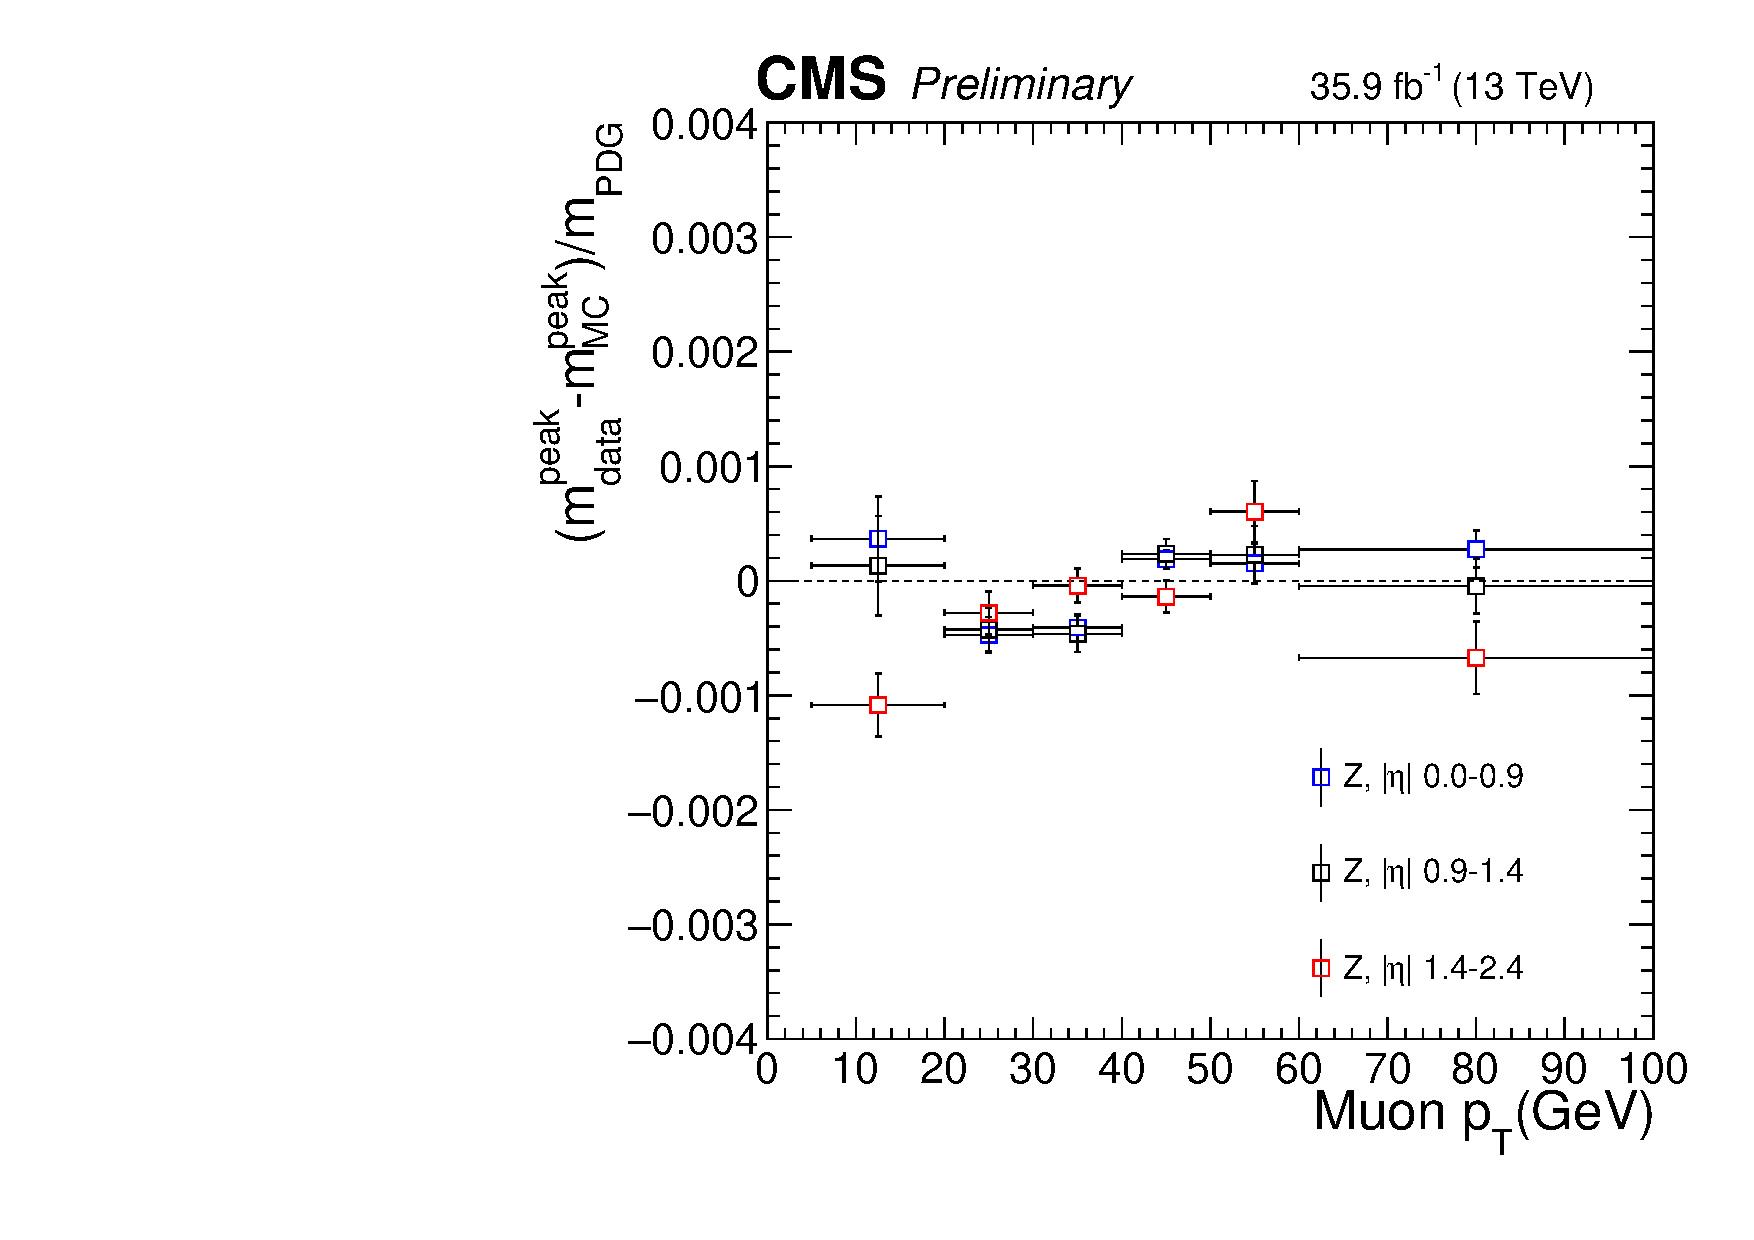
\includegraphics[width=0.44\linewidth]{Figures/Results/mass/lepScale_vs_pt_eta_mu.pdf}
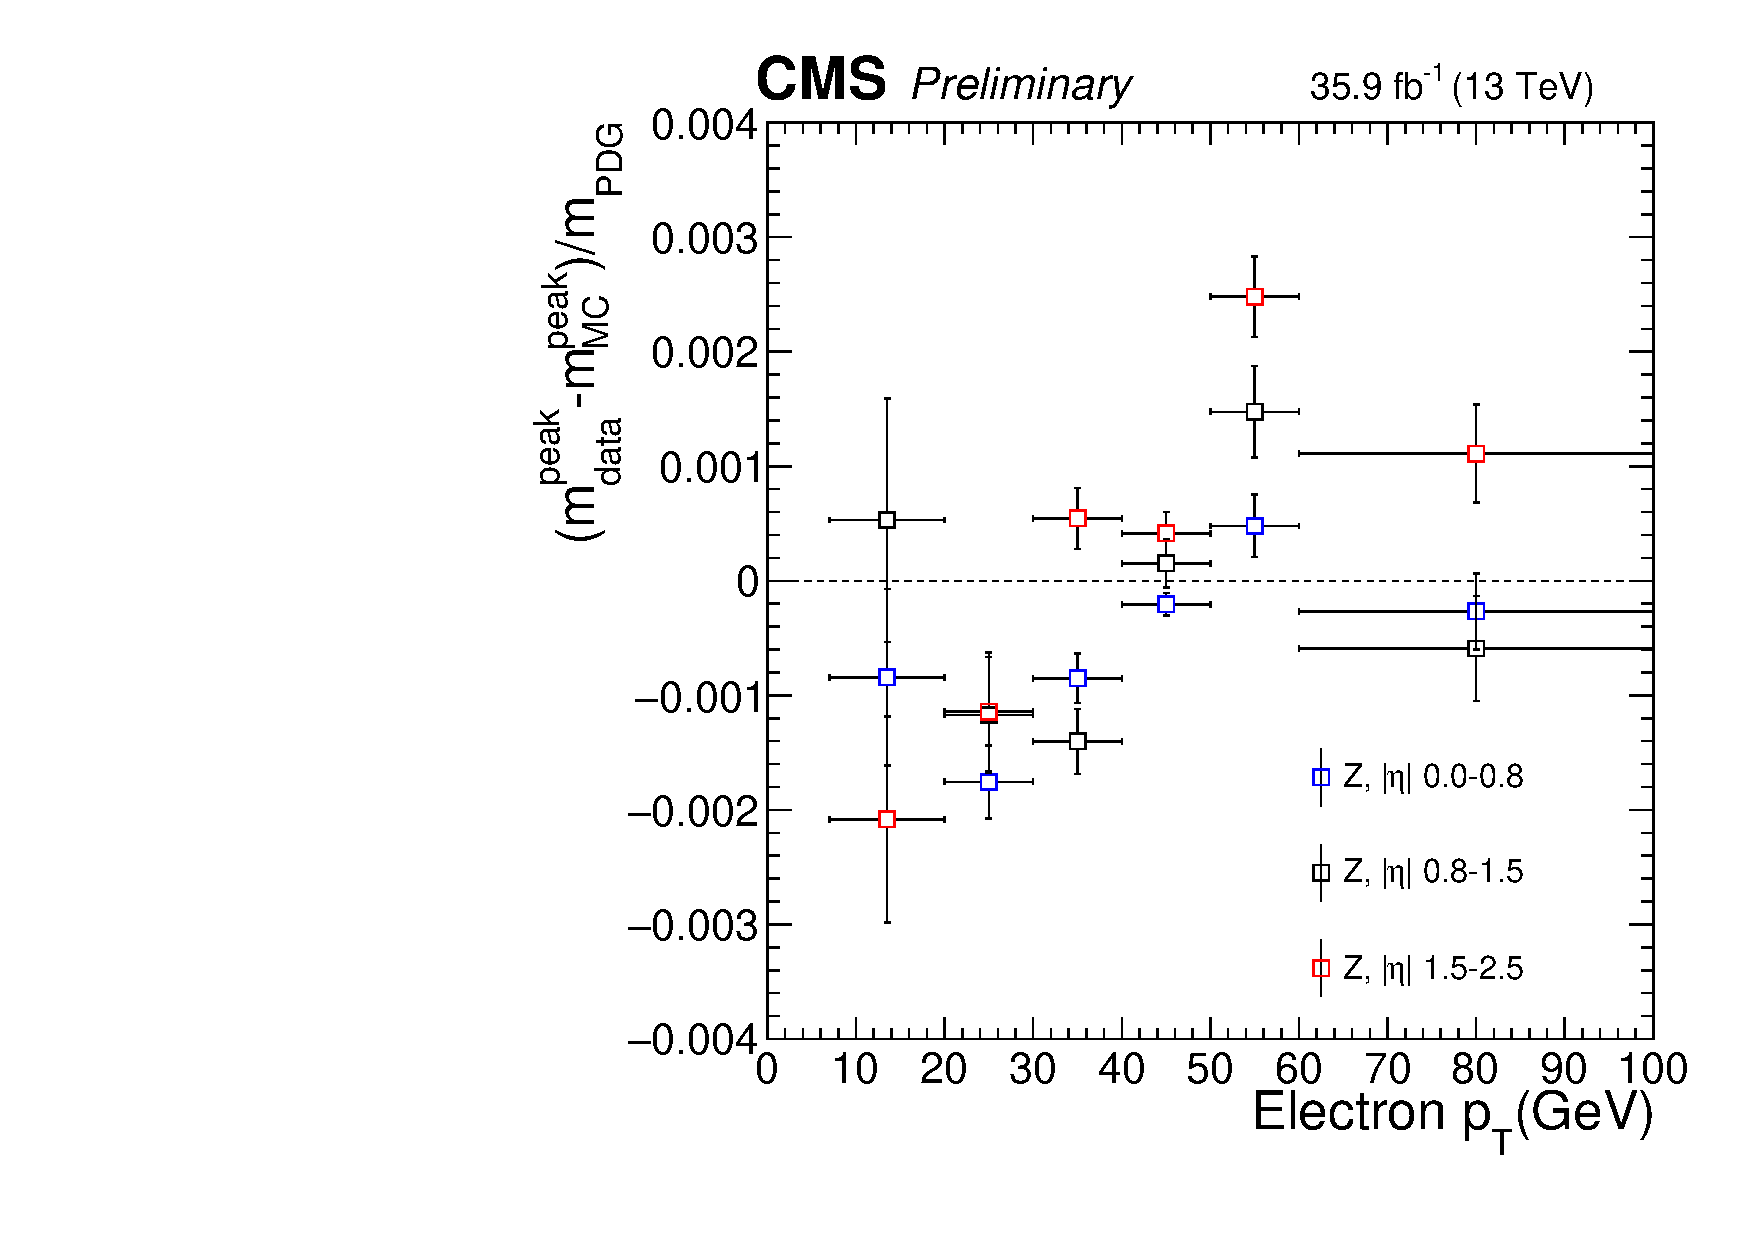
\includegraphics[width=0.44\linewidth]{Figures/Results/mass/lepScale_vs_pt_eta_e.pdf}
\caption{ Difference between the ${\rm Z}\rightarrow\ell\ell$ mass peak positions in data and simulation normalized by the 
nominal $\cPZ$ boson mass obtained as a function of the $\pt$ and $|\eta|$ of one of the leptons regardless of the second
for muons (left) and electrons (right).
\label{fig:lepScale}}
\end{center}
\end{figure}

\begin{figure}[!htb]
\begin{center}
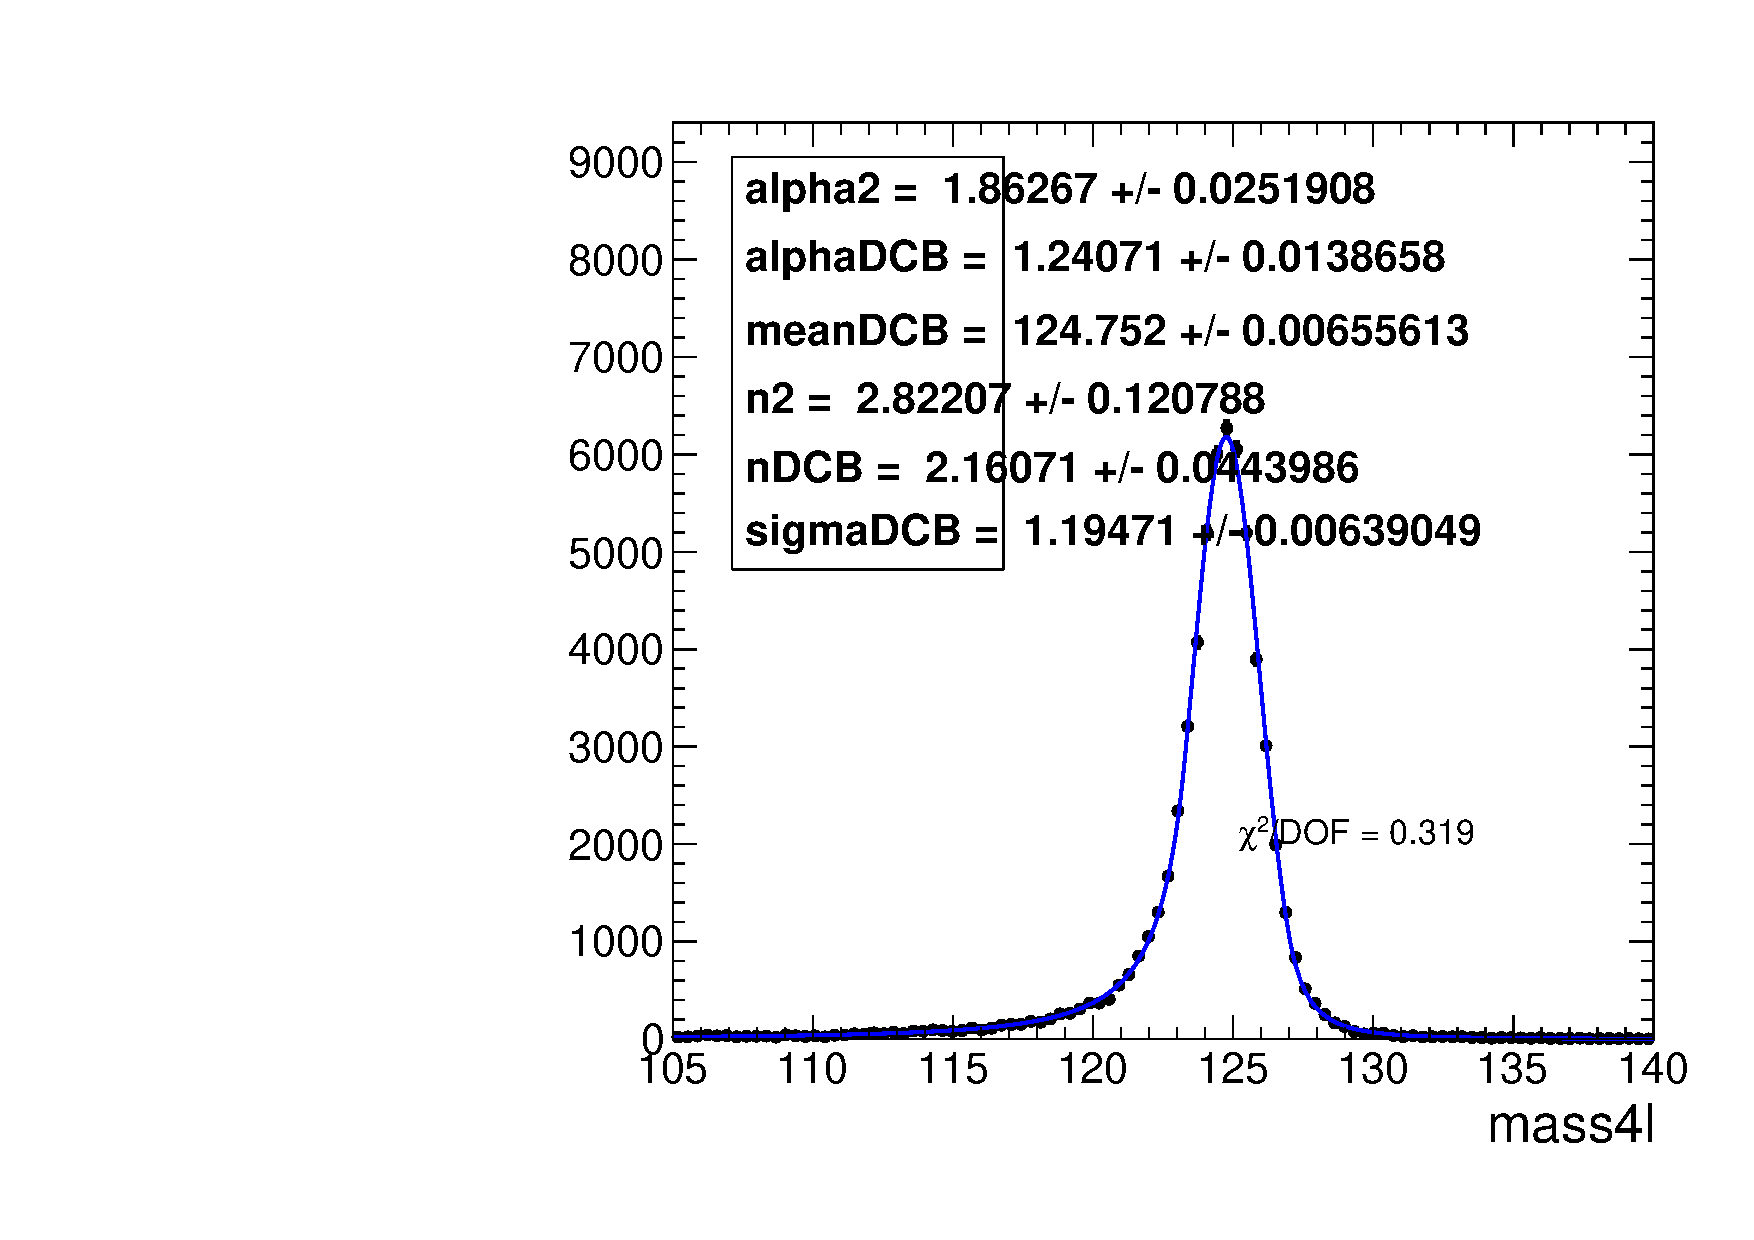
\includegraphics[width=0.32\linewidth]{Figures/Results/mass/m4lreco_4mu_dn.pdf}
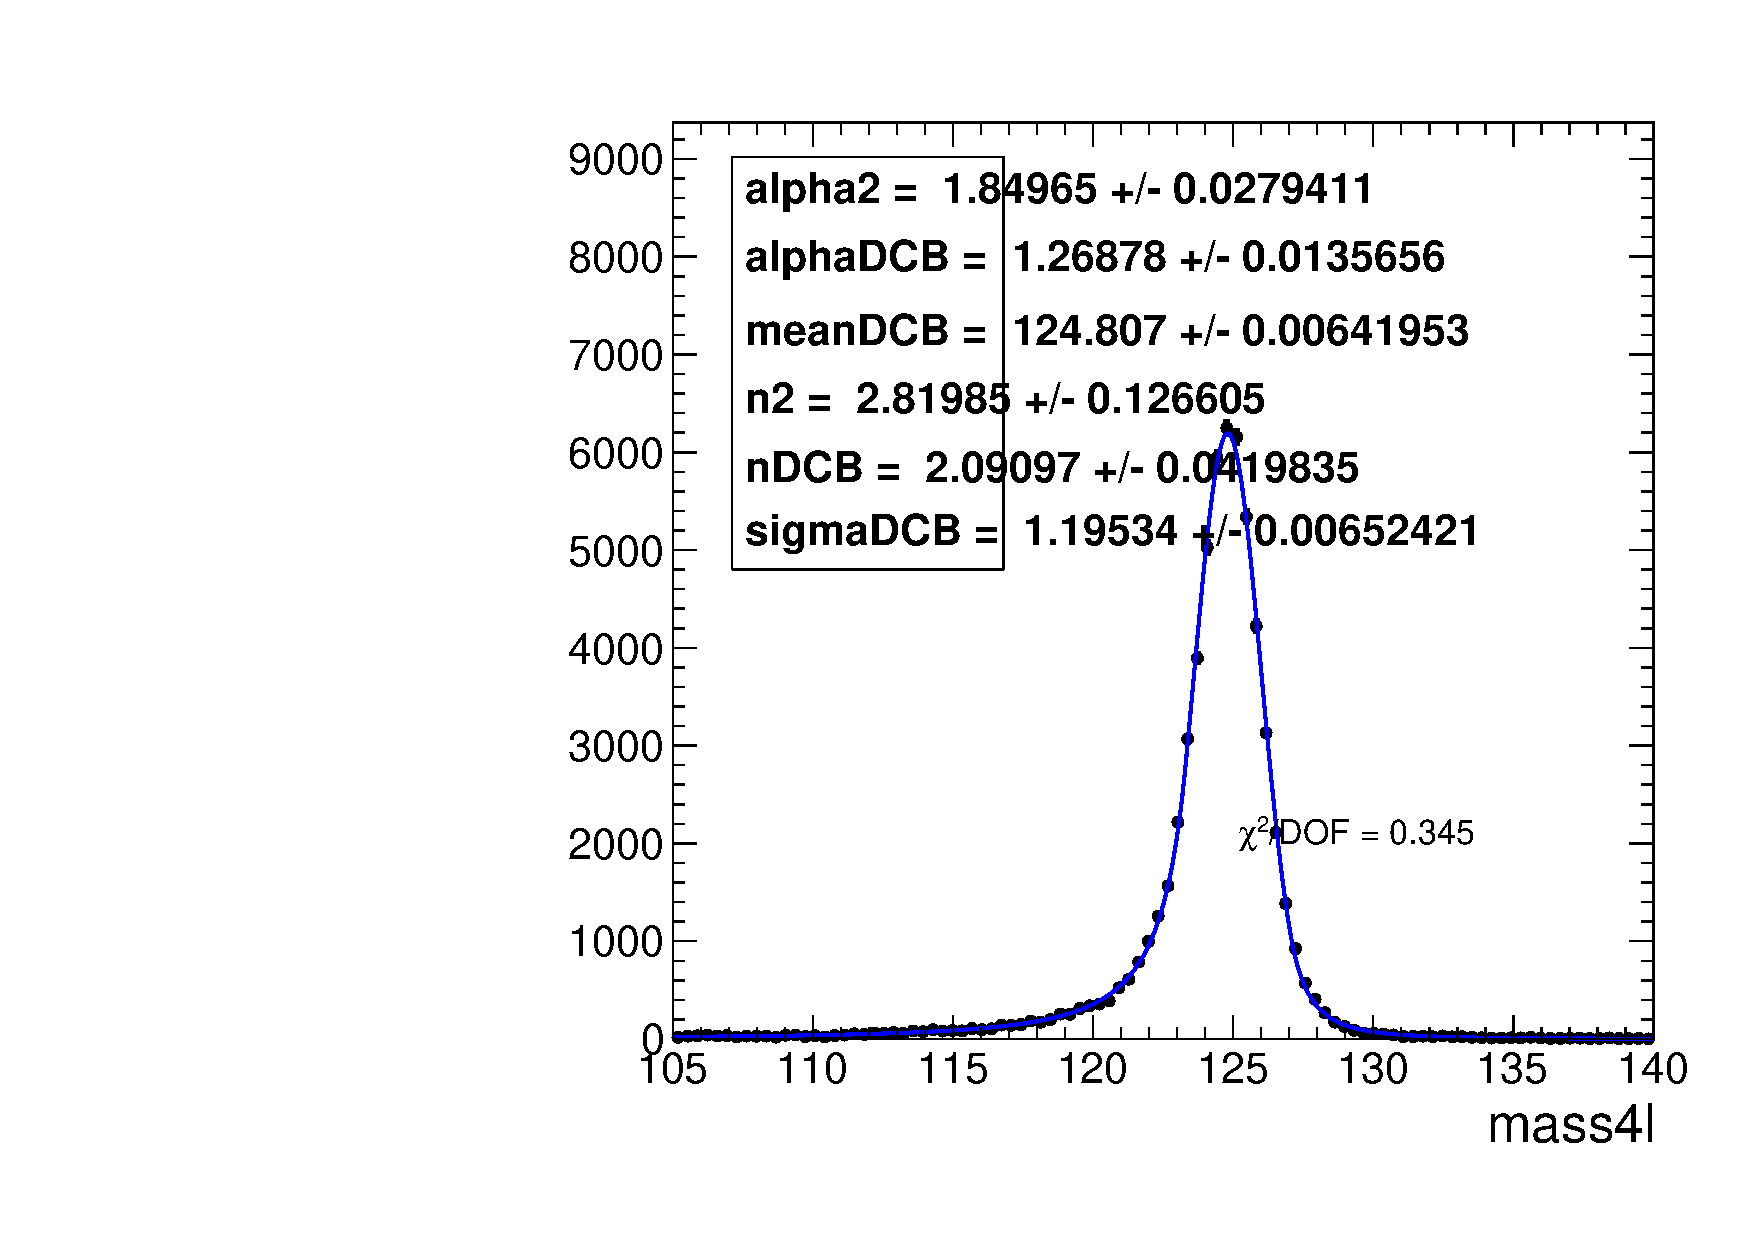
\includegraphics[width=0.32\linewidth]{Figures/Results/mass/m4lreco_4mu.pdf}
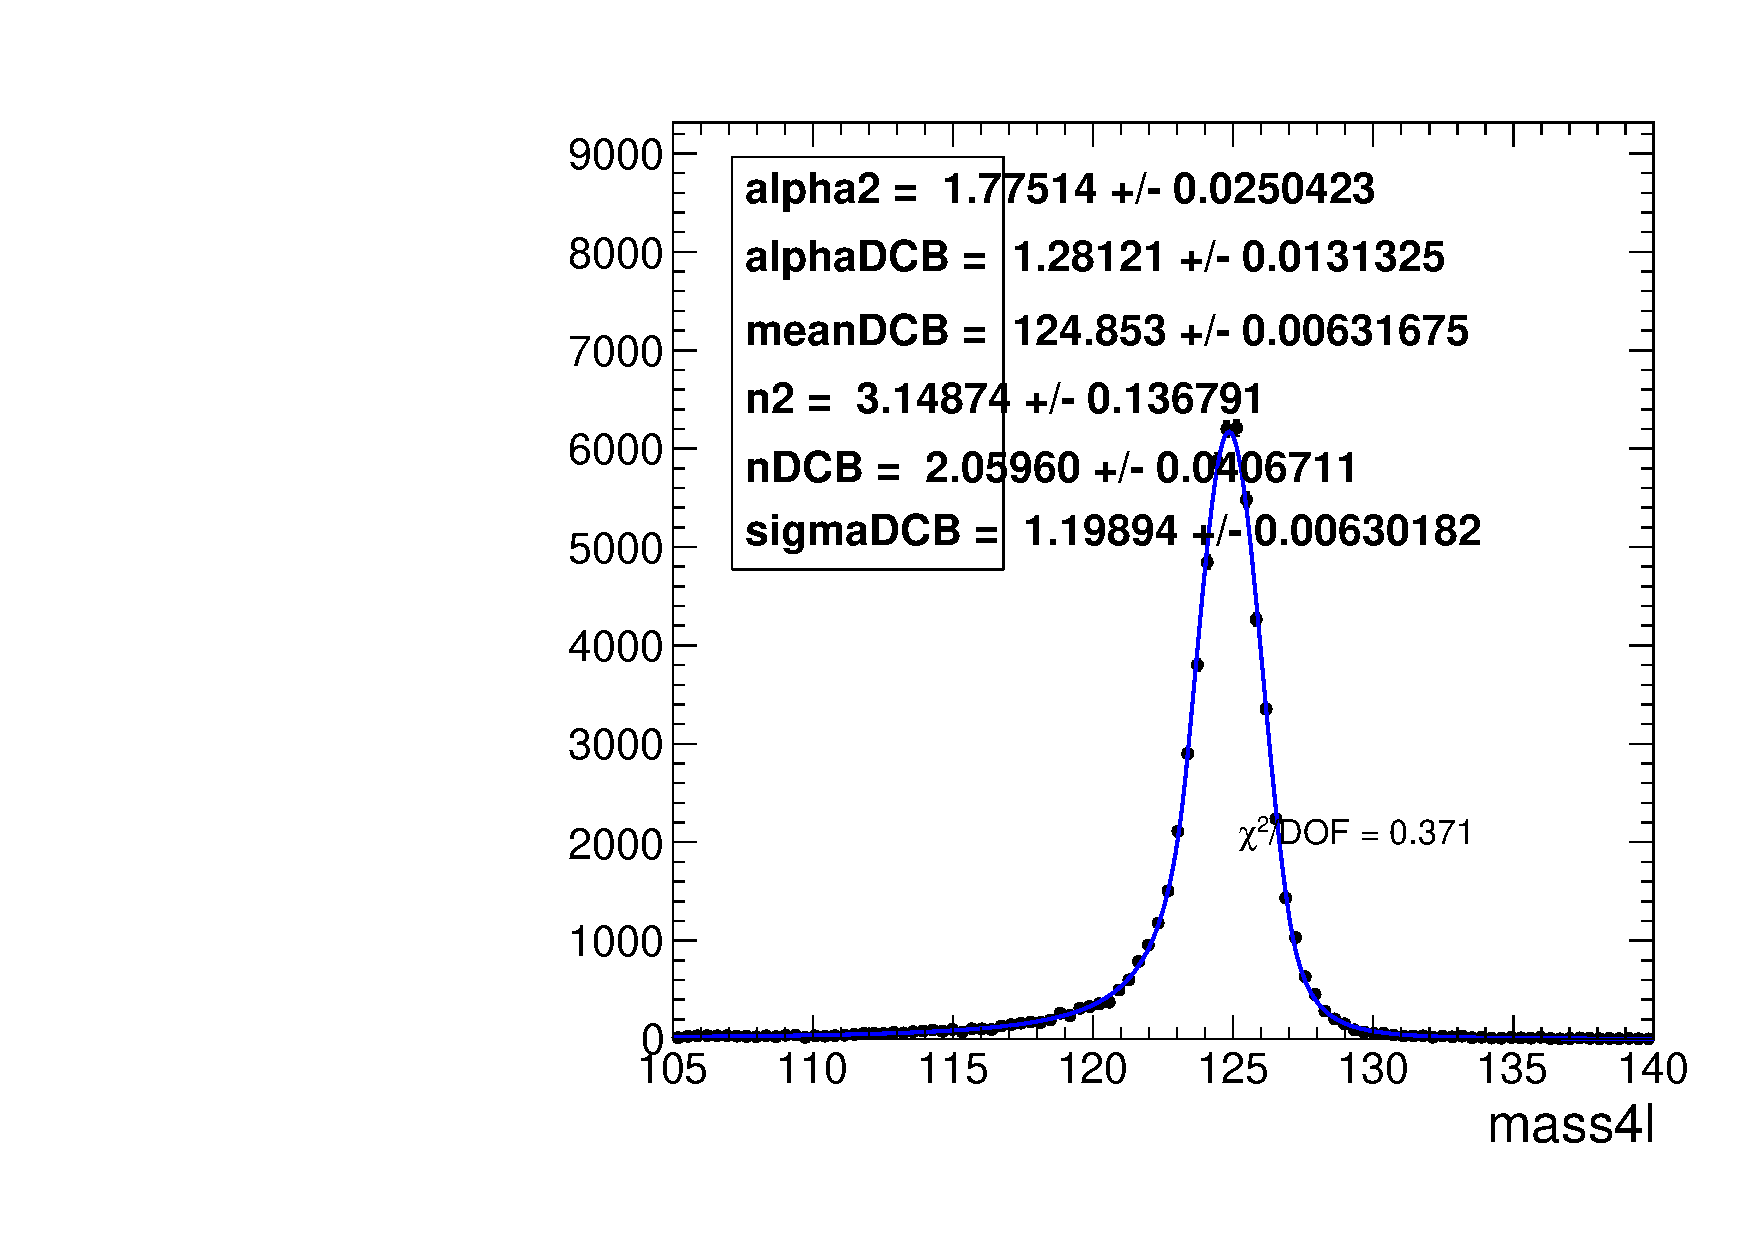
\includegraphics[width=0.32\linewidth]{Figures/Results/mass/m4lreco_4mu_up.pdf} \\
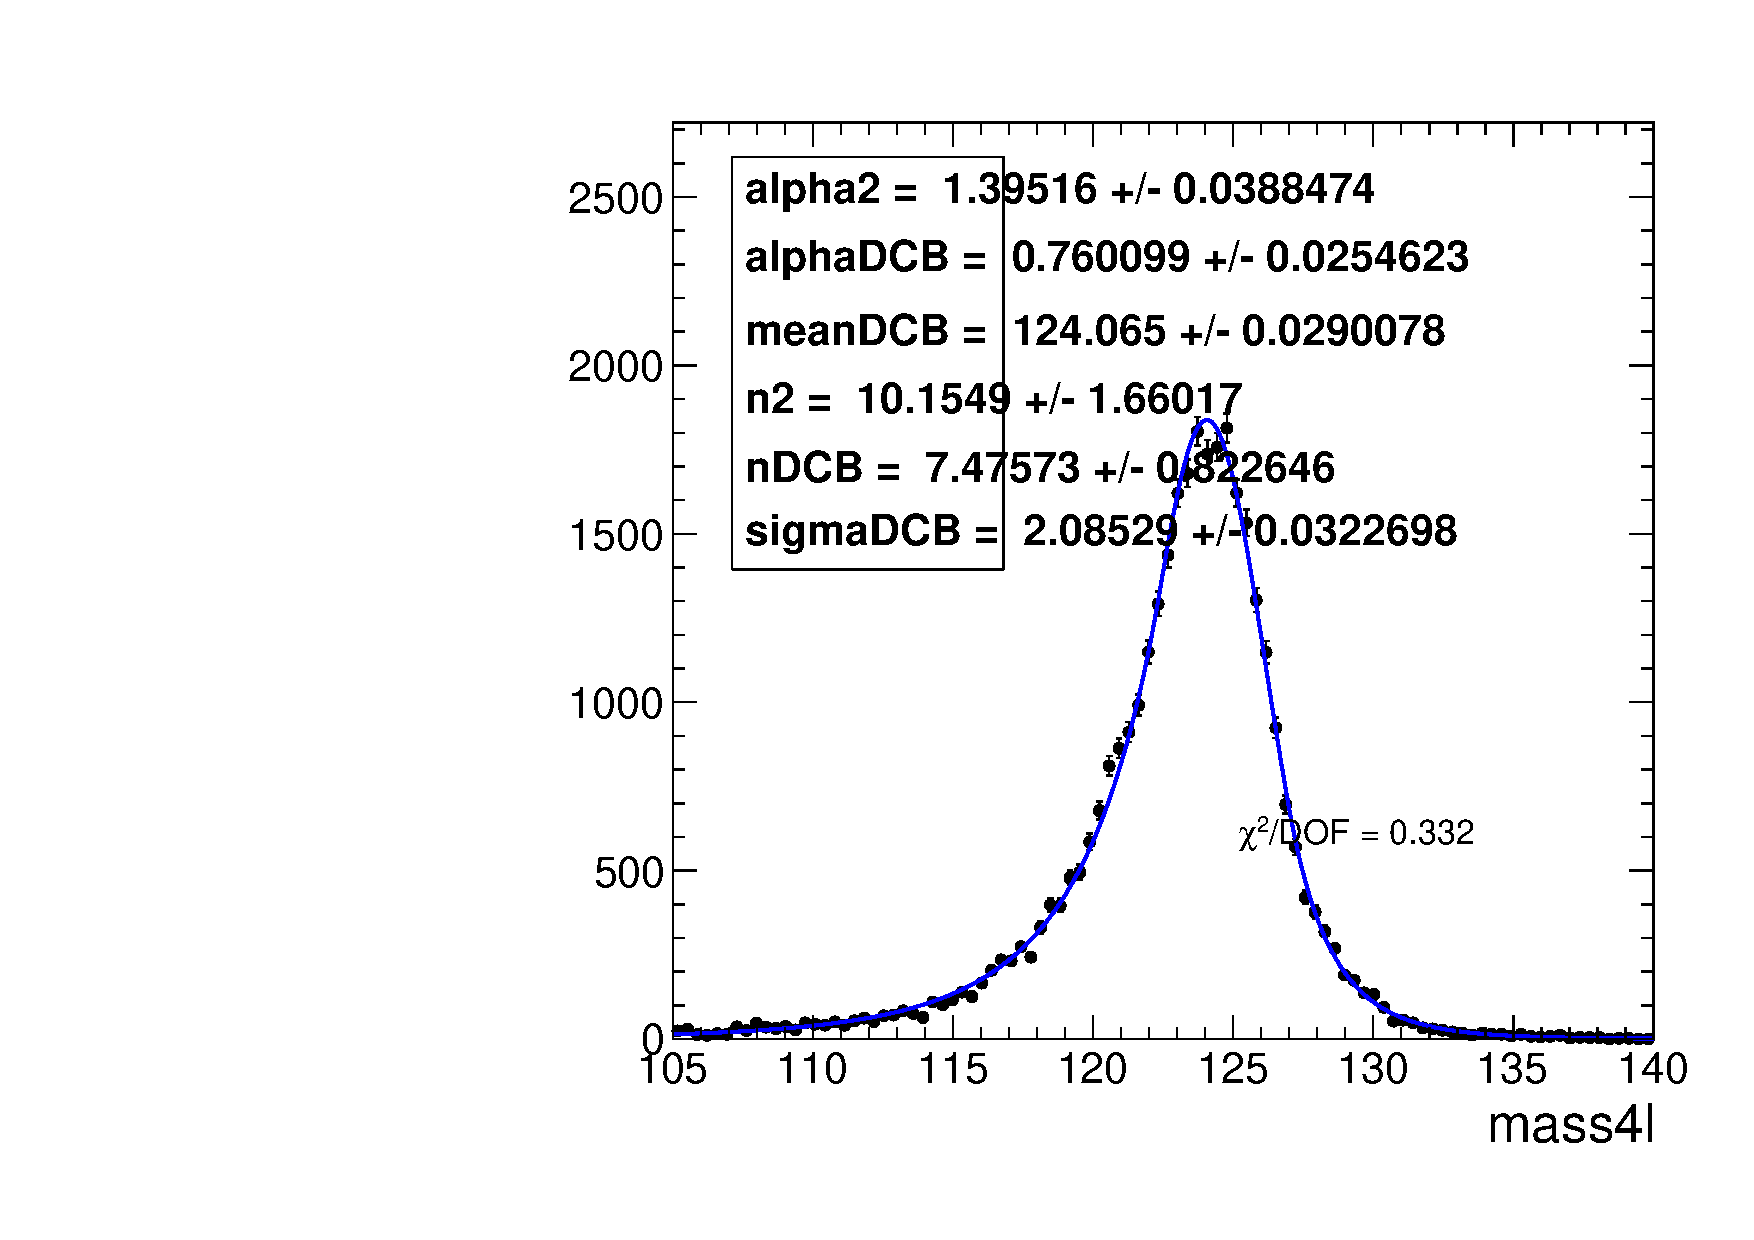
\includegraphics[width=0.32\linewidth]{Figures/Results/mass/m4lreco_4e_dn.pdf}
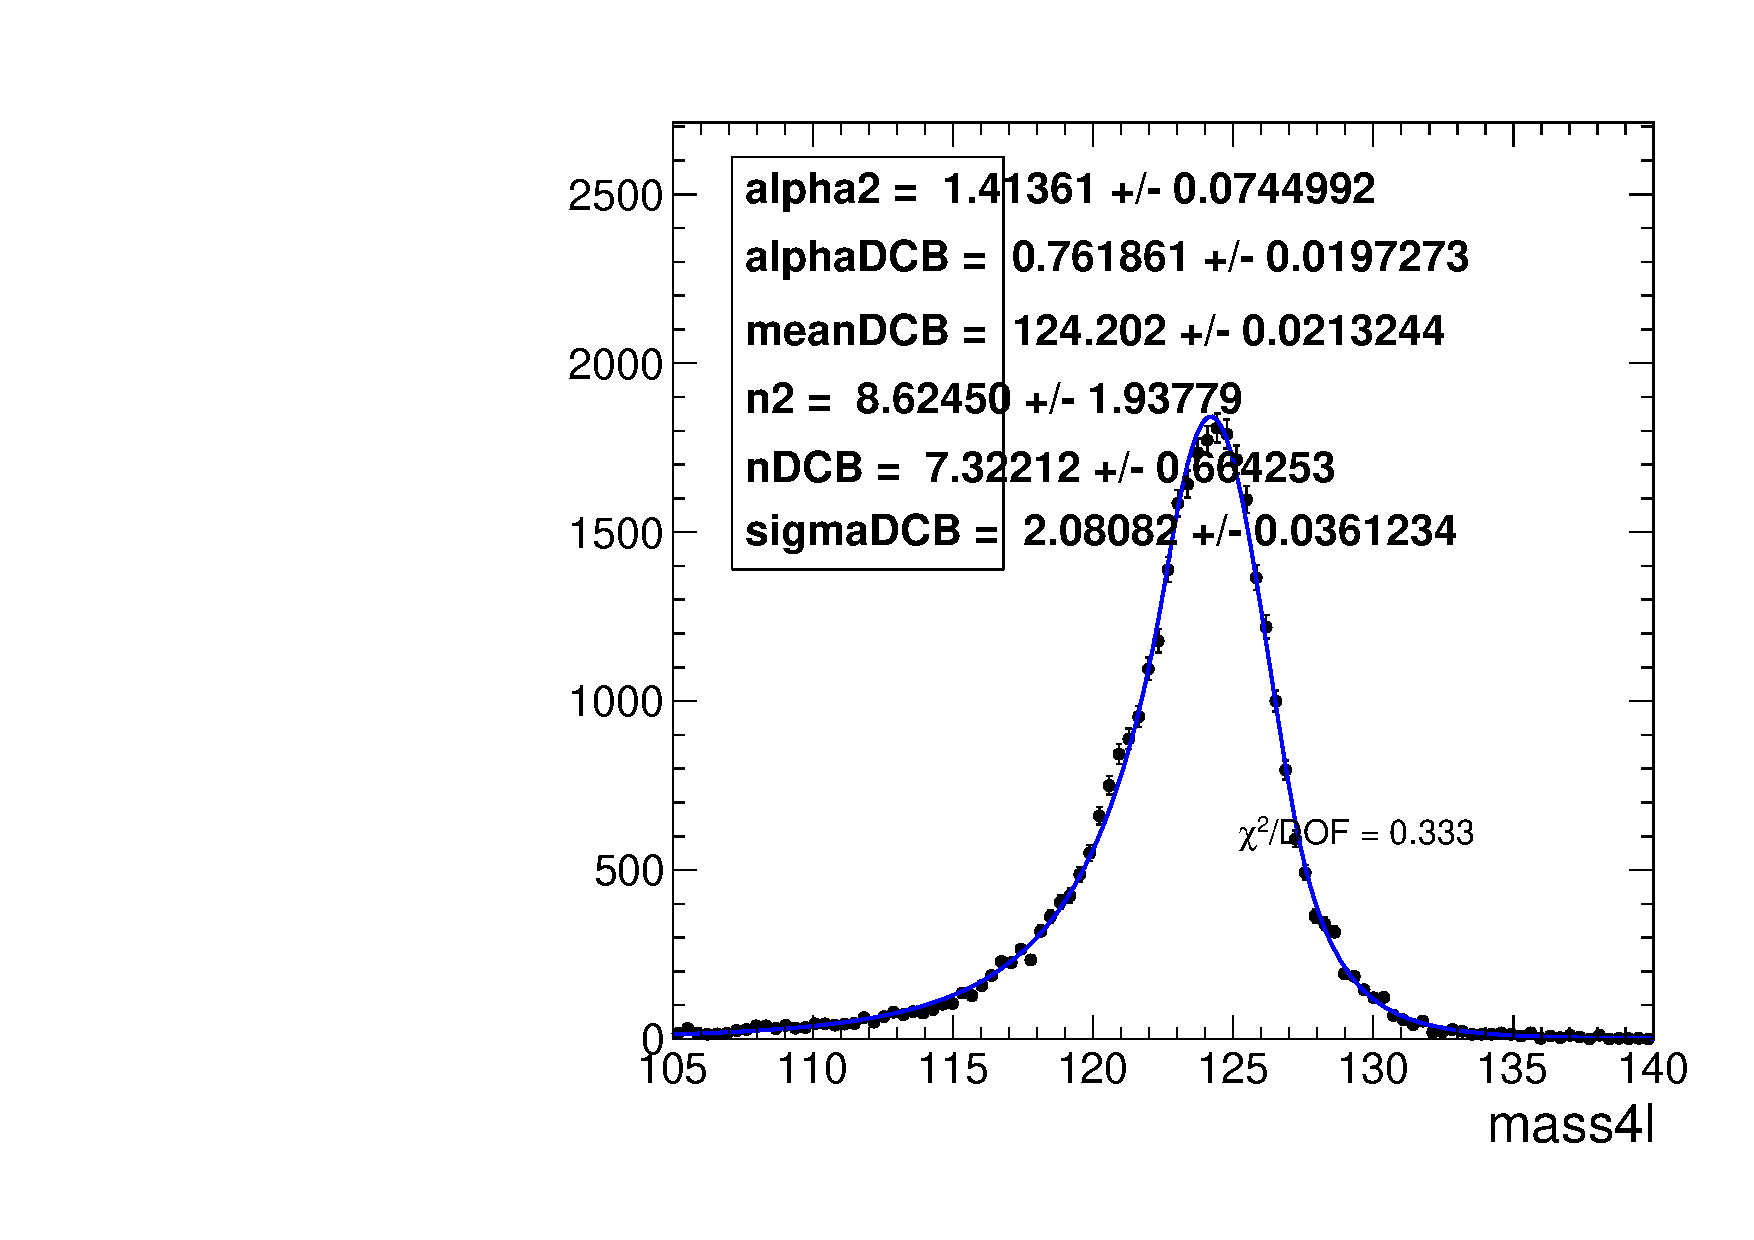
\includegraphics[width=0.32\linewidth]{Figures/Results/mass/m4lreco_4e.pdf}
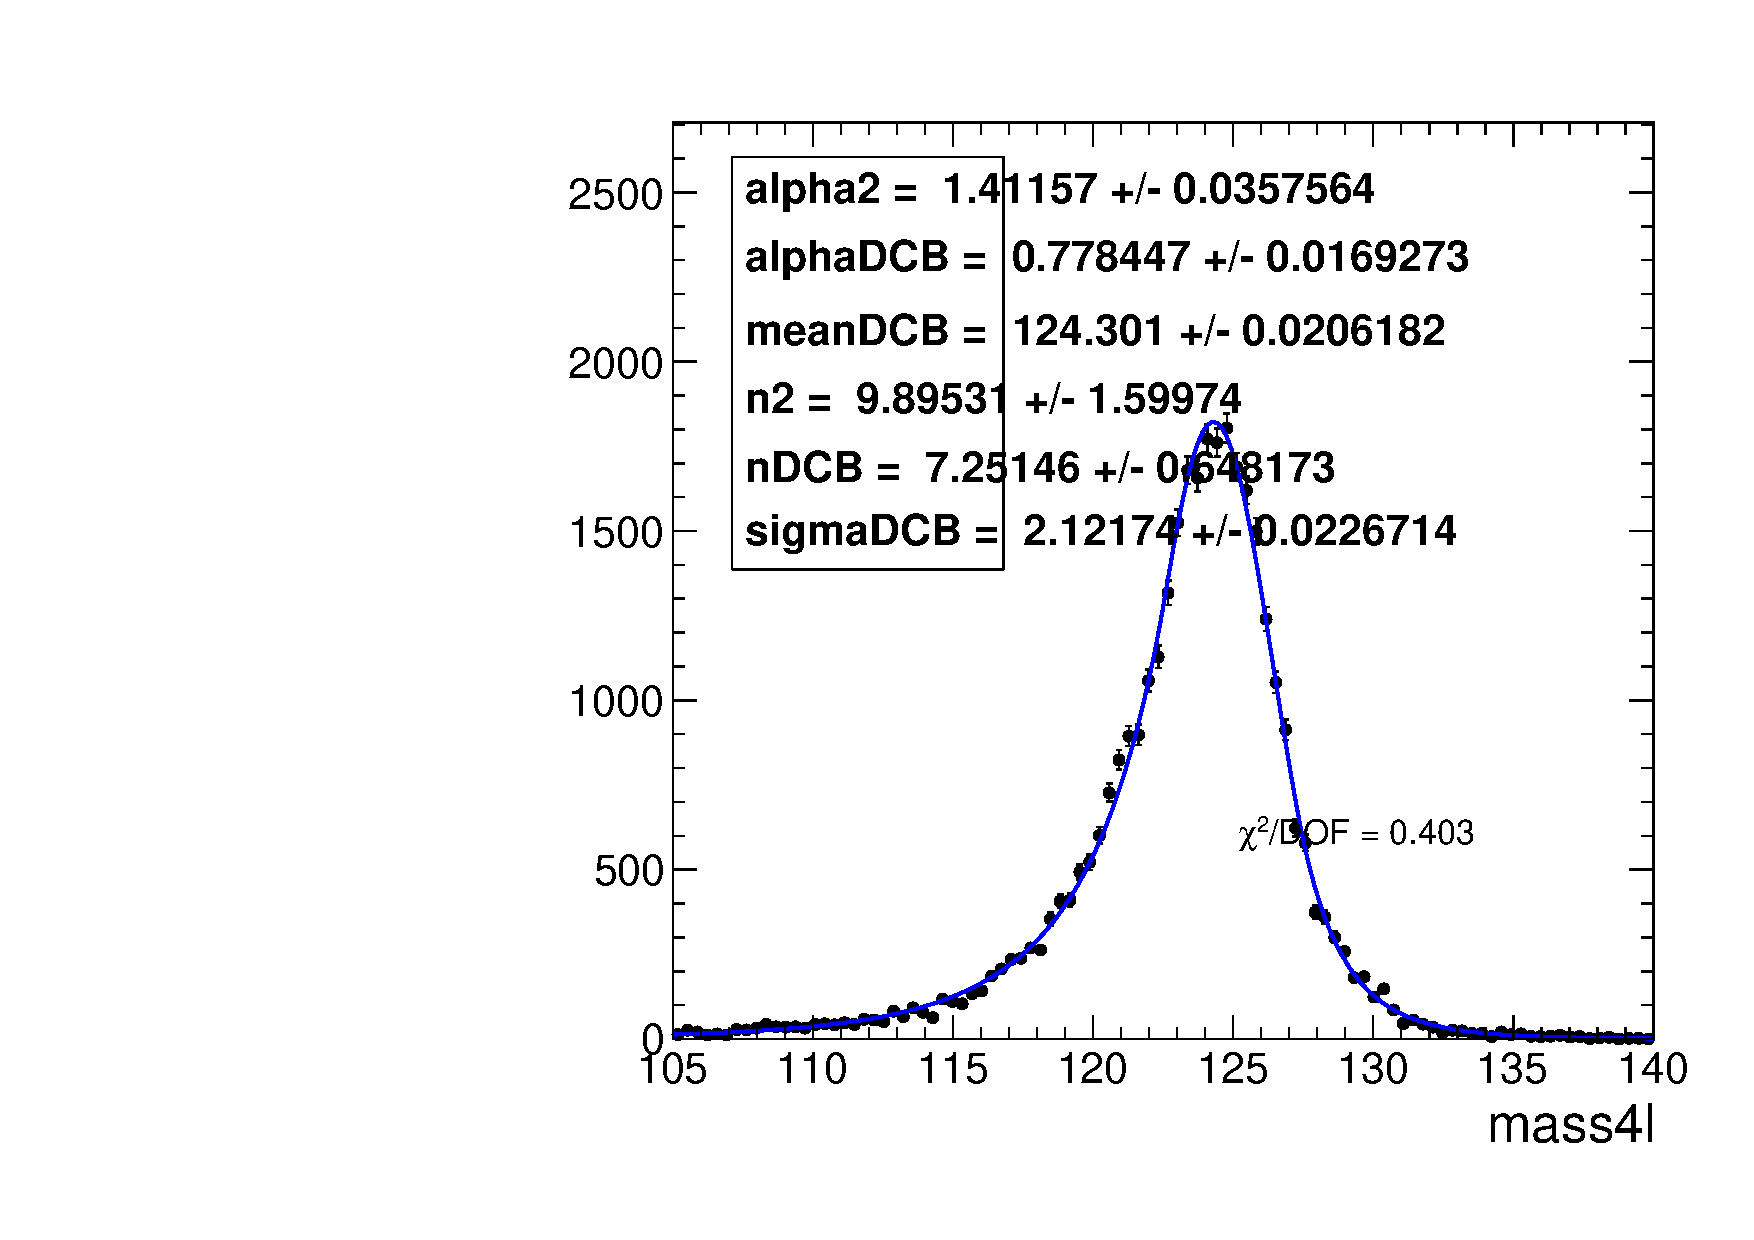
\includegraphics[width=0.32\linewidth]{Figures/Results/mass/m4lreco_4e_up.pdf} 
\caption{ Different $\mllll$ distributions after propagating the biases in Fig.~\ref{fig:lepScale} to Higgs boson events. The change in the mean of the 
double crystal ball is used to determine the systematic uncertainty due to the lepton momentum scale. The middle plot shows the nominal distribution, while
the left (right) plots show the down (up) systematic variations. The $4\mu$ channel is shown in the top row and the $4e$ channel is shown in the bottom row.
\label{fig:lepScaleM4l}}
\end{center}
\end{figure}

Theoretical uncertainties which affect both the background signal and background estimation 
include uncertainties from the renormalization and factorization scale and choice of PDF set. 
The uncertainty from the renormalization and factorization scale is determined by varying these scales between 
0.5 and 2 times their nominal value while keeping their ratio between 0.5 and 2. 
The uncertainty from the PDF set is determined 
by taking the root mean square of the variation when using different replicas of the default NNPDF set. An additional
uncertainty of the 10\% on the K factor used for the $\ggZZ$ prediction is applied as described in Section~\ref{sec:irrbkgd}.
A systematic uncertainty of 2\% on the branching ratio of $\HZZfl$ only affects the signal yield. 
In the case of event categorization, experimental and theoretical uncertainties which account for
possible migration of signal and background events between categories are included. The main sources 
of uncertainty on the event categorization include the QCD scale, PDF set, and the modeling of hadronization and the underlying 
event. These uncertainties amount to between 4--20\% for the signal and 3--20\% for the background depending on the category.
The lower range corresponds to the VBF and VH processes and the upper range corresponds to the $\ggH$ process yield in the VBF-2jet-tagged category. 
Additional uncertainties come from the imprecise knowledge of the jet energy scale (from 2\% for the $\ggH$ yield in the untagged category to 15\% for  $\ggH$ yield in the VBF-2jet-tagged category) and b-tagging efficiency and mistag 
rate (up to 6\% in the -tagged category). 
%rate (up to 6\% in the $\ttH$-tagged category). 


\begin{table}[!htb]
\begin{center}
\small
\caption{
Summary of the experimental systematic uncertainties in the $\Hllll$ measurements. %Details about the derivation of each uncertainty can be found in the text.
\label{tab:SystOverview}
}
\begin{tabular}{|lc|} 
\hline %---------------------------------------------------------
\hline %---------------------------------------------------------
\multicolumn{2}{|c|}{\textbf{Summary of relative systematic uncertainties}} \\
\hline %---------------------------------------------------------
\hline %---------------------------------------------------------
\multicolumn{2}{|c|}{Common experimental uncertainties} \\
\hline %---------------------------------------------------------
\vspace{-0.4cm} & \\
Luminosity & 2.6 \%  \\ 
\vspace{-0.4cm} & \\
Lepton identification/reconstruction efficiencies & 2.5 -- 9 \% \\ 
%\vspace{-0.4cm} & \\
\hline %---------------------------------------------------------
\hline %---------------------------------------------------------
\multicolumn{2}{|c|}{Background related uncertainties} \\
\hline %--------------------------------------------------------
\vspace{-0.4cm} & \\
Reducible background (Z+X) & 36 -- 43 \% \\ 
% \vspace{-0.4cm} & \\
% Event categorization (experimental) & 2 -- 15 \% \\ 
% Event categorization (theoretical) & 3 -- 20 \% \\ 
%\vspace{-0.4cm} & \\
\hline %---------------------------------------------------------
\hline %---------------------------------------------------------
\multicolumn{2}{|c|}{Signal related uncertainties} \\
\hline %---------------------------------------------------------
\vspace{-0.4cm} & \\
Lepton energy scale & 0.04 -- 0.3 \% \\ 
\vspace{-0.4cm} & \\
Lepton energy resolution & 20 \% \\ 
% \vspace{-0.4cm} & \\
% Event categorization (experimental) & 2 -- 15 \% \\ 
% Event categorization (theoretical) & 4 -- 20 \% \\ 
%\vspace{-0.4cm} & \\
\hline %---------------------------------------------------------
\hline %---------------------------------------------------------
\end{tabular}
\normalsize
\end{center}
\end{table}



\begin{table}[!htb]
\begin{center}
\small
\label{tab:SystOverviewTheo}
\caption{Summary of the theory systematic uncertainties in the $\Hllll$ measurements for the inclusive analysis}
\begin{tabular}{|lc|}
\hline %---------------------------------------------------------
\hline %---------------------------------------------------------
\multicolumn{2}{|c|}{\textbf{Summary of inclusive theory uncertainties}} \\
\hline %---------------------------------------------------------
\hline %---------------------------------------------------------
\vspace{-0.4cm} & \\
QCD scale (${\rm gg}$) & $\pm$ 3.9 \% \\
\vspace{-0.4cm} & \\
PDF set (${\rm gg}$) & $\pm$ 3.2 \% \\
\vspace{-0.4cm} & \\
Bkg K factor (${\rm gg}$) & $\pm$ 10 \% \\
\vspace{-0.4cm} & \\
QCD scale (${\rm VBF}$) & +0.4/-0.3 \% \\
\vspace{-0.4cm} & \\
PDF set (${\rm VBF}$) & $\pm$ 2.1 \% \\
\vspace{-0.4cm} & \\
QCD scale (${\rm WH}$) & +0.5/-0.7 \% \\
\vspace{-0.4cm} & \\
PDF set (${\rm WH}$) & $\pm$ 1.9 \% \\
\vspace{-0.4cm} & \\
QCD scale (${\rm ZH}$) & +3.8/-3.1 \% \\
\vspace{-0.4cm} & \\
PDF set (${\rm ZH}$) & $\pm$ 1.6 \% \\
\vspace{-0.4cm} & \\
QCD scale (${\rm \ttH}$) & +5.8/-9.2 \% \\
\vspace{-0.4cm} & \\
PDF set (${\rm \ttH}$) & $\pm$ 3.6 \% \\
\vspace{-0.4cm} & \\
BR($\HZZfl$) & 2 \% \\
\hline %--------------------------------------------------------
\vspace{-0.4cm} & \\
QCD scale ($\qqZZ$) & +3.2/-4.2 \% \% \\
\vspace{-0.4cm} & \\
PDF set ($\qqZZ$) & +3.1/-3.4 \% \\
\vspace{-0.4cm} & \\
Electroweak corrections ($\qqZZ$) & $\pm$ 0.1 \% \\
\hline %---------------------------------------------------------
\hline %---------------------------------------------------------
\end{tabular}
\normalsize
\end{center}
\end{table}
 
\subsection{Limit setting}

The primary tool used to interpret the analysis described above in the context of the signal models is the HiggsAnalysis-CombinedLimit package \cite{combinetwiki}, a collection of RooStats-based software \cite{roostatstwiki} used within the Higgs PAG \cite{higgspagtwiki}, hereafter called the combine tool, or simply combine. Specifically, limits (one-sided Bayesian credible intervals) are set on the expected and observed signal production cross section times branching ratio BR of H to four leptons for the various benchmarks using the asymptotic $\rm{CL}_S$ method \cite{Cowan:2010js}, an approach to calculating a profile likelihood ratio using an approximation of the LHC test-statistic distributions. The upper limit on the cross section gives the maximum number of events that can be attributed to the signal process, consistant with the data that is observed. Combine finds the upper limit as the numerical solution to Equation~\ref{eq:pCL}, which sets the integral of the posterior probability $p(\sigma|D)d\sigma$ equal to the desired confidence level for the measurement, typicall 95\%. The posterior probability gives the degree of belief that $\sigma$ lies in the interval $[\sigma,\ \sigma+d\sigma]$, and is formed by inverting a multi-Poisson model, $p(D|\sigma,\ \bm{\theta})$ using Bayes' theorem (Equation~\ref{eq:pbayes}), after numerically marginalizing priors describing the uncertainties $\pi(\bm{\theta})$ Equation~\ref{eq:pmarg}.

\begin{equation}\label{eq:pCL}
\int_0^{\sigma_{\rm{Up}}} p(\sigma|D)d\sigma = 1 - \alpha
\end{equation}

\begin{equation}\label{eq:pbayes}
p(\sigma|D) = p(D|\sigma)\pi(\sigma) / p(D)
\end{equation}

\begin{equation}\label{eq:pmarg}
p(D|\sigma) = \int p(D|\sigma,\ \bm{\theta}) \pi(\bm{\theta}) d\bm{\theta}
\end{equation}

Combine takes as input specially formatted text files called data cards, which contain the signal, background, and data yields, along with associated systematic uncertainties, and point to the location of the file containing the shape distributions for each sample. When the shape distributions are included, combine computes the limits accross all bins, then combines the results. So, a non-shape based limit is equivalent to a shape-based limit with one bin. This can be used as a cross check that the shape-based limit is behaving correctly, and to analyze the improvement of using the shape-based approach over non-shape based. The event yields and systematic uncertainties are discussed later in this section.

Combine returns the 95\% confidence level (CL) expected and observed limits on the signal strength parameter, $\mu$, as well as one and two sigma deviations of the expected limit, where $\mu$ is the signal scale factor in the $\rm{i}^{\rm{th}}$ bin in the mean count, $n_i = \mu * s_i + b_i$, where $s_i$ and $b_i$ are the signal and background yields, respectively.

Limits are set for the three decay channels, 4e, 4$\mu$, and 2e2$\mu$ individually, then combined for the 4l limit. The signal strength parameter gives the ratio of the 95\% CL expected signal yield to the theoretical yield, or more generally,

\begin{equation}\label{eq:mu}
\mu[\sigma_{\rm{norm}}*BR] = \frac{\sigma_{95\% \rm{CL}}*BR}{\sigma_{\rm{norm}}*BR},
\end{equation}

where $\sigma_{\rm{norm}}$ is the cross section used to normalize the signal yields given as input to combine, typically the theoretical production cross section, but also set to 1 pb for comparison to other H decay channels. This formula is used to calculate the 95\% CL cross section times branching ratio, which is the desired output variable. This limit can then be compared to the theoretical cross section times BR. The points where the upper limit is lower than the theory value are interpreted as exclusions.


\section{Cross Section Limits}

After the event selection is optimized and all of the uncertainties are accounted for, limits are set on the signal strength parameter, $\mu$, and presented in two ways. For each model, the limits are shown for $\mu$, to be easily compared with the limits obtained by the other H decay channels, and as cross section limit versus mass plots. These results are found for both the cut-and-count and MVA based strategies. Until the selection is frozen and the data unblinded, only expected limits will be plotted in the SR.

\subsection{Cut-and-count based}

\subsubsection{Zp2HDM}

The 1D slice of mass points fixing $m_{A0} = 300$ GeV is selected for the limits plots since this region has the highest cross section and the largest branching fraction to DM production. The 1D limits are presented for $\mu$ in Figure~\ref{fig:limzp2hdmmu} and $\sigma_{95\% \rm{CL}}*BR$ in Figure~\ref{fig:limzp2hdm}, obtained using the optimized selection given in Section~\ref{cutandcountopt}.  

\begin{figure}[tbh]
\centering
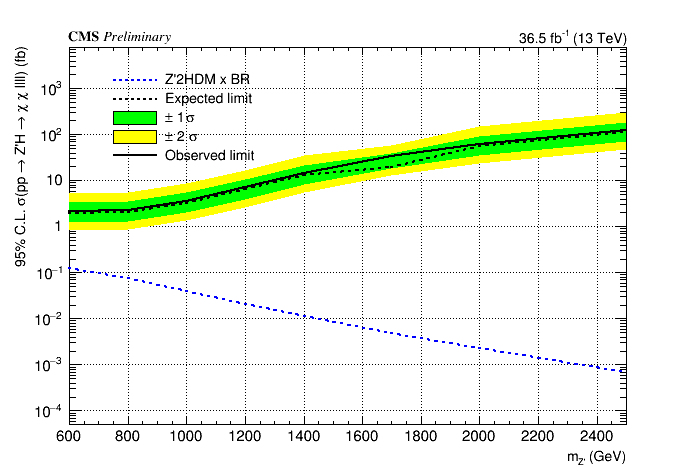
\includegraphics[width=5in]{figures/sigma_limits_4mu_Zp2HDM.png}
\caption{PLACEHOLDER 1D $\mu$ limits for $m_{A0} = 300$ GeV for Zp2HDM.}
\label{fig:limzp2hdmmu}
\end{figure}

\begin{figure}[tbh]
\centering
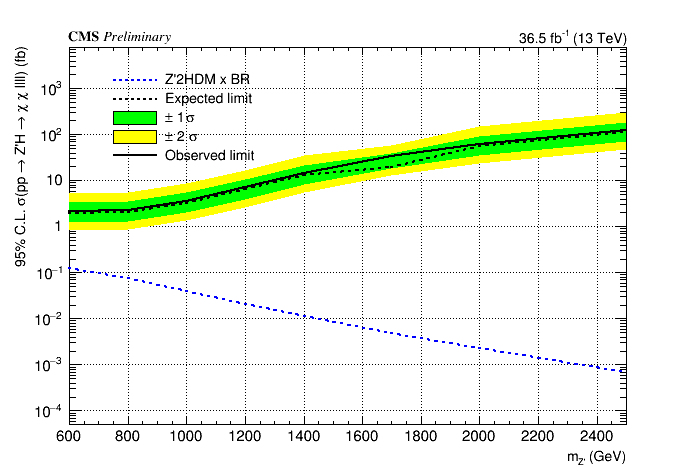
\includegraphics[width=5in]{figures/sigma_limits_4mu_Zp2HDM.png}
\caption{PLACEHOLDER 1D cross section times BR limits for $m_{A0} = 300$ GeV for Zp2HDM.}
\label{fig:limzp2hdm}
\end{figure}

\subsubsection{ZpBaryonic}

The 1D slice of mass points fixing $m_{\chi} = 1$ GeV is selected for the limits plots since this region has the highest cross section. The 1D limits are presented for $\mu$ in Figure~\ref{fig:limzpbaryonicmu} and $\sigma_{95\% \rm{CL}}*BR$ in Figure~\ref{fig:limzpbaryonic}, obtained using the optimized selection given in Section~\ref{cutandcountopt}.  

\begin{figure}[tbh]
\centering
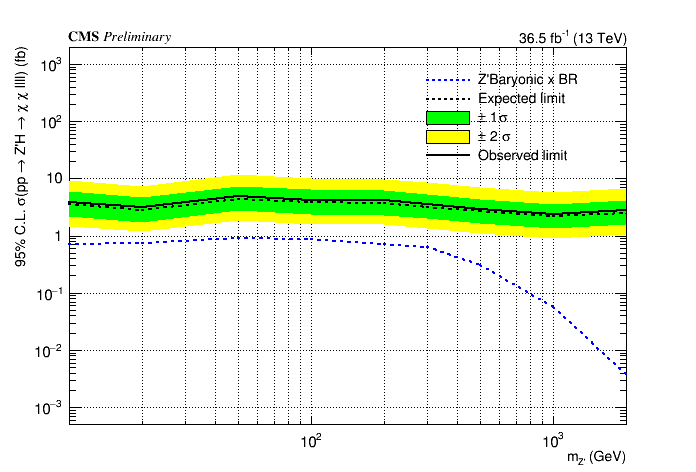
\includegraphics[width=5in]{figures/sigma_limits_4mu_ZpBaryonic.png}
\caption{PLACEHOLDER 1D $\mu$ limits for $m_{\chi} = 1$ GeV for ZpBaryonic.}
\label{fig:limzpbaryonicmu}
\end{figure}

\begin{figure}[tbh]
\centering
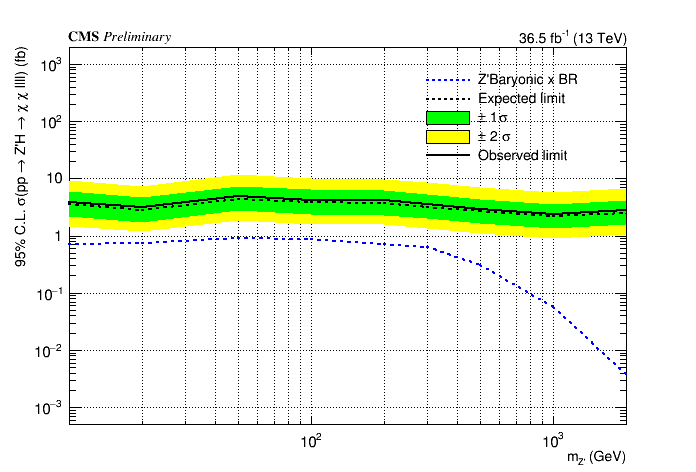
\includegraphics[width=5in]{figures/sigma_limits_4mu_ZpBaryonic.png}
\caption{PLACEHOLDER 1D cross section times BR limits for $m_{\chi} = 1$ GeV for ZpBaryonic.}
\label{fig:limzpbaryonic}
\end{figure}

\subsection{MVA based}

\subsubsection{Zp2HDM}

The 1D limits are presented for $\mu$ in Figure~\ref{fig:limzp2hdmmu} and $\sigma_{95\% \rm{CL}}*BR$ in Figure~\ref{fig:limzp2hdm}, obtained using the optimized selection given in Section~\ref{mvaopt}.

\begin{figure}[tbh]
\centering
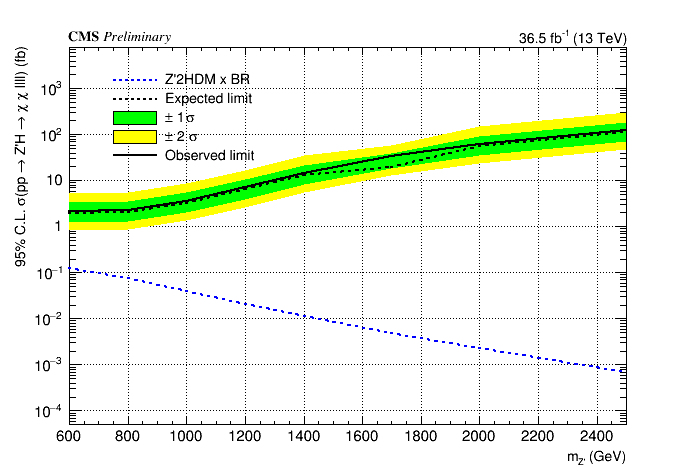
\includegraphics[width=5in]{figures/sigma_limits_4mu_Zp2HDM.png}
\caption{PLACEHOLDER 1D $\mu$ limits for $m_{A0} = 300$ GeV for Zp2HDM.}
\label{fig:limzp2hdmmu}
\end{figure}

\begin{figure}[tbh]
\centering
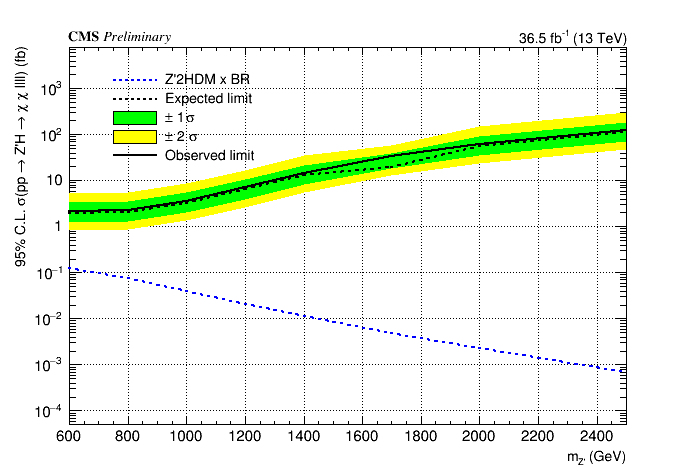
\includegraphics[width=5in]{figures/sigma_limits_4mu_Zp2HDM.png}
\caption{PLACEHOLDER 1D cross section times BR limits for $m_{A0} = 300$ GeV for Zp2HDM.}
\label{fig:limzp2hdm}
\end{figure}

\subsubsection{ZpBaryonic}

The 1D limits are presented for $\mu$ in Figure~\ref{fig:limzpbaryonicmu} and $\sigma_{95\% \rm{CL}}*BR$ in Figure~\ref{fig:limzpbaryonic}, obtained using the optimized selection given in Section~\ref{mvaopt}.

\begin{figure}[tbh]
\centering
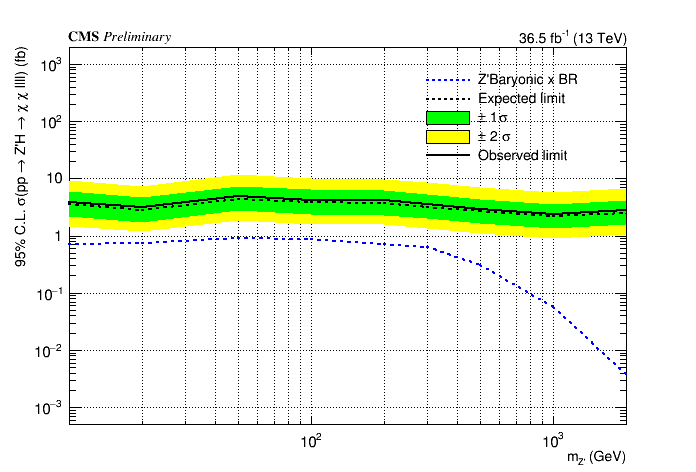
\includegraphics[width=5in]{figures/sigma_limits_4mu_ZpBaryonic.png}
\caption{PLACEHOLDER 1D $\mu$ limits for $m_{\chi} = 1$ GeV for ZpBaryonic.}
\label{fig:limzpbaryonicmu}
\end{figure}

\begin{figure}[tbh]
\centering
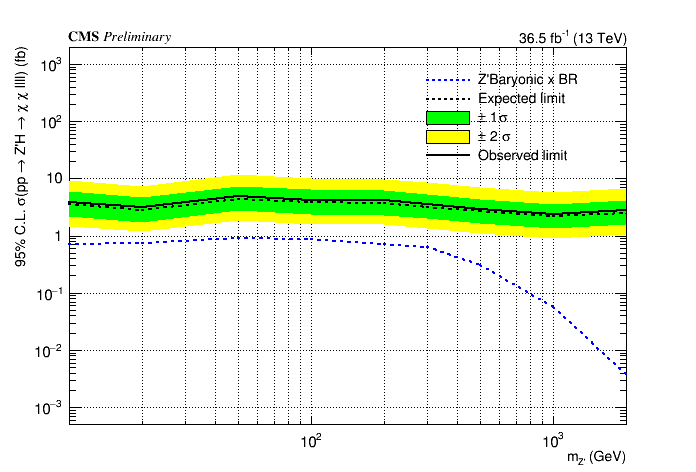
\includegraphics[width=5in]{figures/sigma_limits_4mu_ZpBaryonic.png}
\caption{PLACEHOLDER 1D cross section times BR limits for $m_{\chi} = 1$ GeV for ZpBaryonic.}
\label{fig:limzpbaryonic}
\end{figure}


